\chapter{Risk Assessment}

	The risk assesment table is our base criteria for total risk assessment. The table tells 
	the risk of different combinations of consequence and probability. The consequence and 
	probability is ranked High, Medium and Low. 

		\begin{figure}[H]
			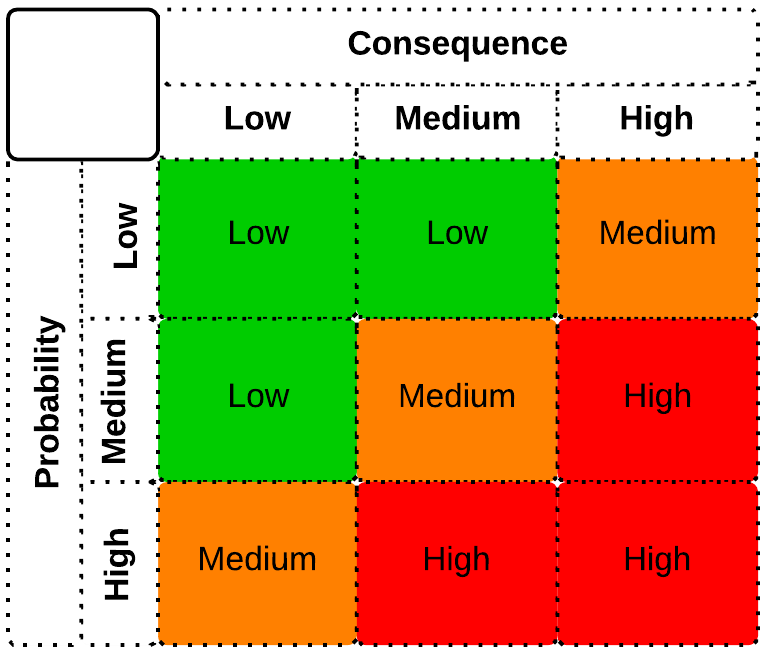
\includegraphics[scale=0.3]{pics/risk.png}
		\end{figure}

	In the following tables we have performed a risk identification and a risk assessment for 
	each separate use case. In the risk identification we have evaluated each function and 
	considered what may go wrong. In addition we have evaluated where in the source code the 
	error may occur. For each use case and risk assessment, we have rated the risk for the customer, 
	the user and the developer. 

	\clearpage

	\section{Scenario 1}
	

	\section{Scenario 2}

	\section{Scenario 3}

	\section{Scenario 4}
